\section{Introduction}
\label{section:intro}
In multi-tenant datacenters, VMs play an integral role by enabling a diverse set of operating systems and
software to be run on a unified underlying framework. However, out-dated, inefficient, 
or misconfigured TCP stacks can be implemented in the VMs. 
In this paper, we explore how operators can regain control of TCP's congestion control, 
regardless of the TCP stack
running in a VM. Our aim is to allow a cloud provider to utilize advanced TCP stacks, such as DCTCP~\cite{alizadeh2011data}, 
without having control over the VM or requiring changes in network hardware.
We propose a scheme that exerts fine-grained
control over arbitrary tenant TCP stacks by enforcing per-flow congestion
control in the virtual switch. 
%Our scheme is light-weight, flexible, scalable and can police non-conforming flows. 
%Our evaluation shows the computational overhead of LiquidSwitch is less than 4\% and implementing an administrator-defined congestion control algorithm
%in the vSwitch (\ie{}, DCTCP) closely tracks its native performance, regardless of the VM's TCP stack.


\section{Our Approach}
%Figure~\ref{acdc_highlevel} shows the high-level structure of \acdc{}.
We present \acdc{}, a new technology that implements
TCP congestion control within a vSwitch to help ensure VM
TCP performance cannot impact the network in an adverse way. At a high-level (Figure~\ref{acdc_highlevel}), the vSwitch monitors all packets for a flow, modifies
packets to support features not implemented in the VM's TCP stack (\eg{}, ECN) and reconstructs
important TCP parameters for congestion control.~\acdc runs the congestion control logic specified by an administrator and then enforces an intended
congestion window by modifying the receiver advertised window (\rwnd{}) on incoming ACKs. A policing
mechanism ensures stacks cannot benefit from ignoring~\rwnd{} and can also be used for non-TCP traffic.
\begin{figure}[!t]
        \centering
  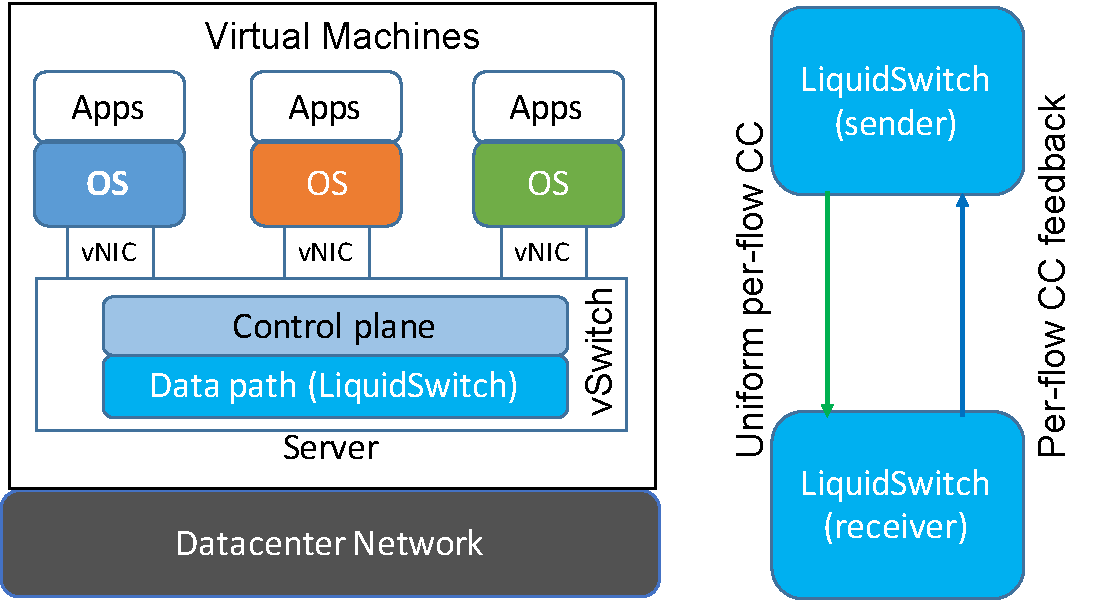
\includegraphics[width=0.35\textwidth]{figures/acdc_highlevel_long.pdf}
        \caption{\acdc{} high-level architecture.}
        \label{acdc_highlevel}
\end{figure}

~\acdc allows for
administrators to enforce a uniform, network-wide congestion control algorithm without changing VMs. DCTCP congestion control algorithm is implemented in \acdc{}, this allows for high throughput and low latency, regardless of the congestion control algorithms VMs use. Furthermore,
our system mitigates the impact of varying TCP stacks running on the same fabric. This improves fairness and additionally
solves the ECN co-existence problem identified in production networks~\cite{wu2012tuning,judd2015nsdi}.
LiquidSwitch is easy to implement, computationally lightweight, scalable and modular.
% so that it is highly complimentary to
%performance isolation schemes also designed for virtualized datacenter environments.

\section{Experiment Results}
\begin{figure}[t]
        \centering
        \begin{subfigure}[b]{0.225\textwidth}
                \centering
                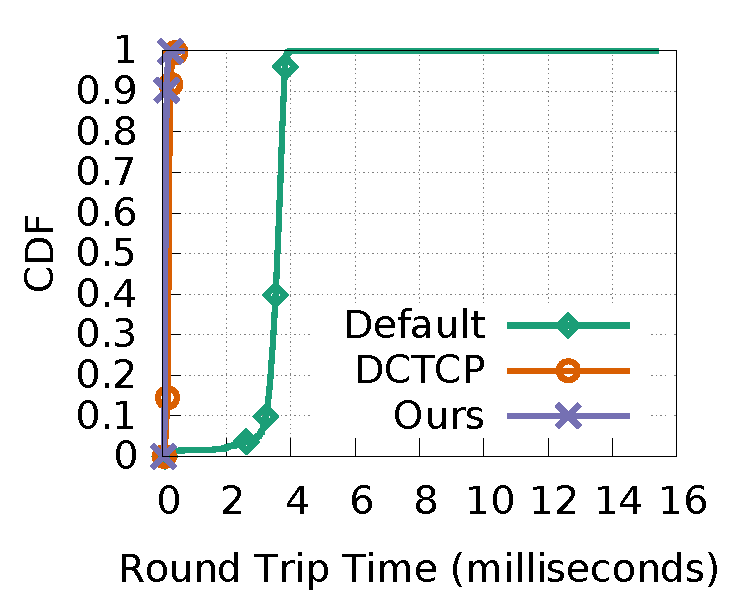
\includegraphics[width=\textwidth]{./figures/incast/16to1/incast_16to1_test_sockperf.pdf}
                \caption{TCP RTT in 16-to-1 incast.}
                \label{rtt}
        \end{subfigure}
        \begin{subfigure}[b]{0.225\textwidth}
                \centering
                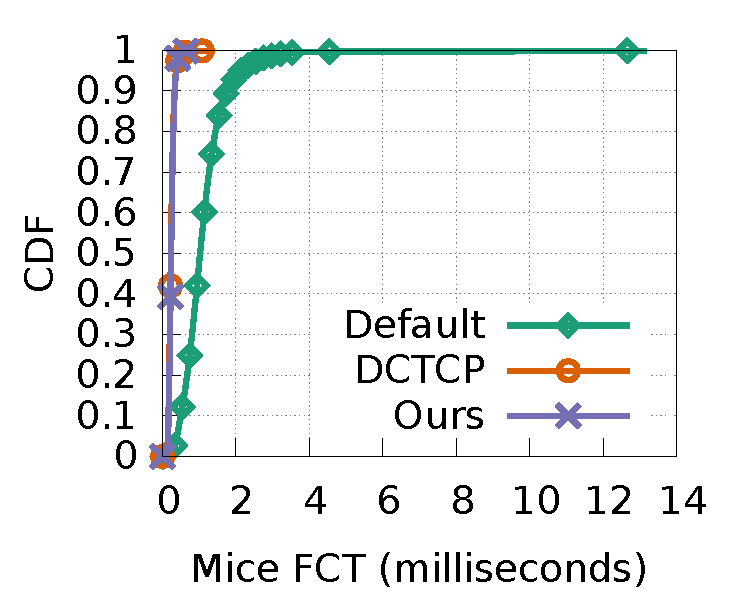
\includegraphics[width=\textwidth]{./figures/macro_benchmarks/macro_4stride/stride4_mice16KB_fct.pdf}
                \caption{mice flow (16KB) FCT in concurrent stride test.}
                \label{fct}
        \end{subfigure}
        \caption{LiquidSwitch Performance}
        \label{performance}
\end{figure}
We attach 17 servers to a IBM G8264 10Gbps switch. We measure Default (CUBIC stack without ECN) and DCTCP (ECN-enabled) on an unmodified vSwitch. We compare them to LiquidSwitch (CUBIC on host with LiquidSwitch-based vSwitch).
Our evaluation (Figure~\ref{performance}) shows \acdc{} closely tracks DCTCP's performance regardless of the VM's TCP stack and outperforms Default.
The computational overhead of \acdc{} is less than 4\% compared with the baseline case.
